\subsection{The Nagel-Schreckenberg model}
This model was created in the 90s by the German physicists Kai Nagel and Michael Schreckenberg to simulate 
traffic flow on highways. It explained the so called \textit{Phantom-Congestion} which occurs when drivers 
linger by not accelerating even if they have the opportunity to do so.

The model is a cellular automata based on four very simple rules, which are applied in sequence. One complete loop is called an iteration.

\begin{enumerate}
\item Acceleration: Each vehicle, that has not yet reached the maximum speed (which is 5), increases its speed by one unit.
\item Deceleration: If the size of the gap (in cells) between two vehicles is less than the speed of the following car (in speed units), this cars speed is reduced to a value equivalent to the size of the gap.
\item Lingering: Every vehicle reduces its speed by 1 with a probability $p$ $(0 \leq p \leq 1)$.
\item Moving forward: Every vehicle moves forward the number of cells equal to its speed.
\end{enumerate}

\subsection{Example of an iteration}
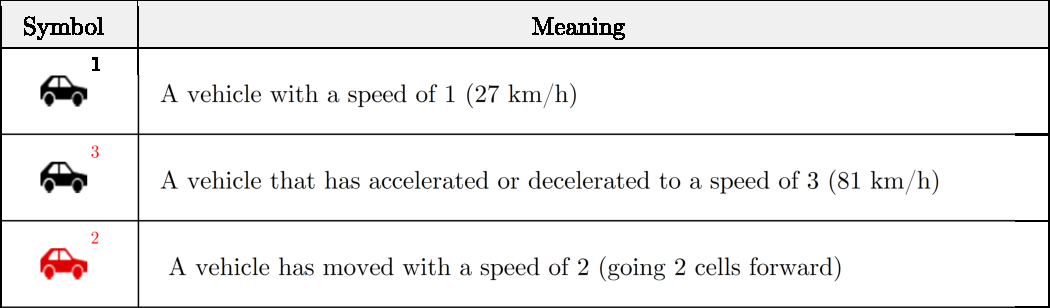
\includegraphics[width=\textwidth]{nasch_symbol.pdf} \vspace*{1cm}

Random startup setting for time \textit{t}\\ \vspace{-.2cm}

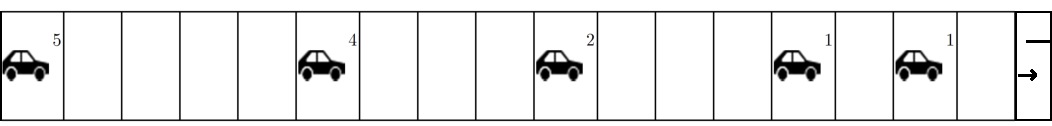
\includegraphics[width=\textwidth]{nasch_1.pdf}\vspace*{1cm}

Step (1) -- Acceleration, $v_{max} = 5$\\ \vspace{-.2cm}

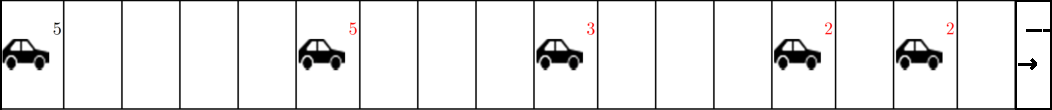
\includegraphics[width=\textwidth]{nasch_2.pdf}\vspace*{1cm}

Step (2) -- Deceleration\\ \vspace{-.2cm}

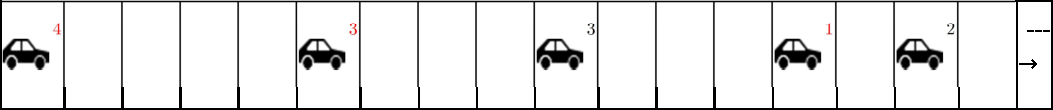
\includegraphics[width=\textwidth]{nasch_3.pdf}\vspace*{1cm}

Step (3) -- Lingering ($\rho = 1/3$, affecting the two leading cars)\\ \vspace{-.2cm}

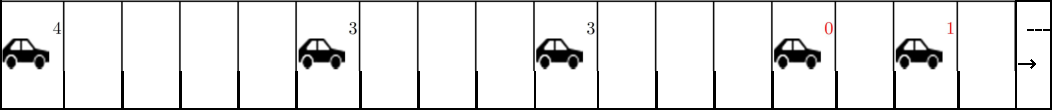
\includegraphics[width=\textwidth]{nasch_4.pdf}\vspace*{1cm}

Step (4) -- Moving (Setting for the time \textit{t + 1})\\ \vspace{-.2cm}

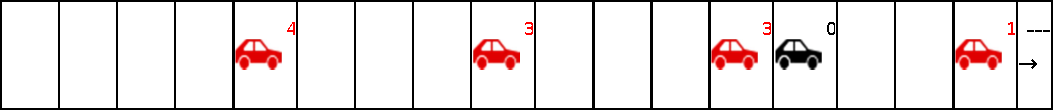
\includegraphics[width=\textwidth]{nasch_5.pdf}


\subsection{Situation}
The distance between Erstfeld and the Gotthard tunnel is relevant for the model. The highway to the tunnel is two-laned and will be reduced to one lane in front of the tunnel. As on the figure \ref{sketch} shown, the authors resigned to depicted any exits. The reason for this is first to reduce complexity of the model and second to neglect irrelevant factors. In case of congestion there is a red light that regulates the traffic flow, that is also took in account in the model. 

\begin{figure}[h]\centering
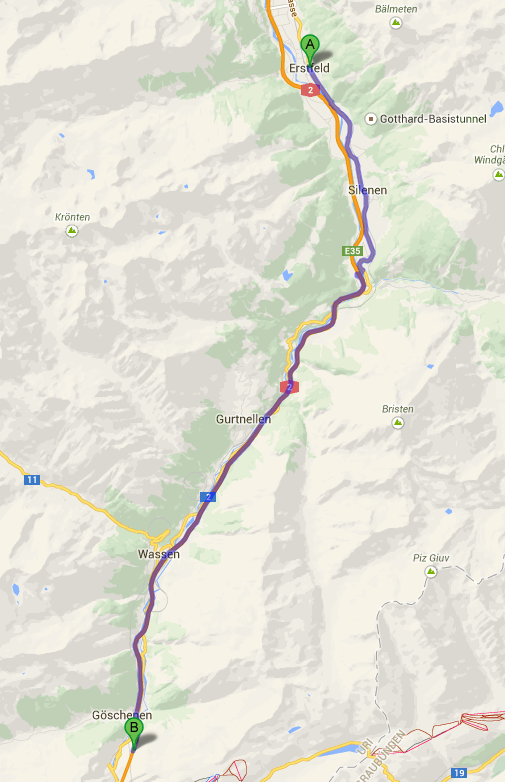
\includegraphics[angle=90, width=.7\textwidth]{map.png}
\caption{map of Uri, A: Erstfeld, B: Gotthard tunnel at Göschenen}
\label{map}
\end{figure}

\begin{figure}[h]\centering
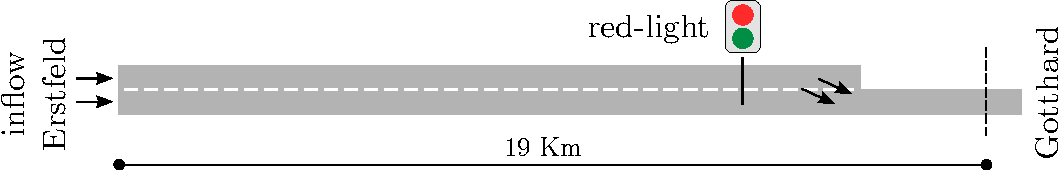
\includegraphics[width=.9\textwidth]{sketch.pdf}
\caption{Sketch of model}
\label{sketch}
\end{figure}